% Preamble
\documentclass{beamer}
\usepackage[spanish]{babel}

% Packages
\usepackage{amsmath}
\usepackage[utf8]{inputenc}
\usepackage[T1]{fontenc}
\usepackage{graphicx}
\usepackage{algorithmicx}
\usepackage{algpseudocode}
\usepackage{caption}
\usepackage{courier}

\captionsetup{justification=centering, font={scriptsize}, skip=0pt}

\usetheme[compress]{Berlin}
\setbeamertemplate{page number in head/foot}[framenumber]

\title[Autómatas Celulares]{Autómatas Celulares: Bandadas de Agentes Autopropulsados}
\subtitle{72.25 - Simulación de Sistemas}
\author[Flores Lucey, Llanos]{Alejo Flores Lucey\inst{1} \and Nehuén Gabriel Llanos\inst{2}}
\institute[Instituto Tecnológico de Buenos Aires]
{
    \inst{1}
    \href{mailto:afloreslucey@itba.edu.ar}{afloreslucey@itba.edu.ar}\\
    Legajo 62622
    \and
    \inst{2}
    \href{mailto:nllanos@itba.edu.ar}{nllanos@itba.edu.ar}\\
    Legajo 62511
}
\date{2024 1C | Grupo Nº3}
\titlegraphic{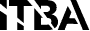
\includegraphics[height=0.5cm]{./itba}}

\makeatletter
\beamer@theme@subsectionfalse
\makeatother

\AtBeginSection[]{
    \begin{frame}
        \begin{beamercolorbox}[sep=8pt,center]{title}
            \usebeamerfont{title}\insertsection
        \end{beamercolorbox}
    \end{frame}
}

\begin{document}

    \begin{frame}
        \titlepage
    \end{frame}

    \begin{frame}{Outline}
        \tableofcontents
    \end{frame}

    \section{Introducción}

        \begin{frame}{Introducción}
            \begin{itemize}
                \item El objetivo es representar el comportamiento de un sistema de partículas autopropulsadas
                (Off Lattice) en un espacio bidimensional.
                \item La implementación del modelo permite simular el sistema de partículas y su interacción.
                \item Se definen observables para el comportamiento del sistema ante ciertos parámetros.
            \end{itemize}
        \end{frame}

        \subsection{Sistema Real}

            \begin{frame}{Sistema Real}
                \begin{itemize}
                    \item El modelo Off Lattice busca analizar el movimiento de un conjunto de partículas y cómo se
                    produce un efecto de agrupamiento cuando interactúan entre sí.
                \end{itemize}
                \begin{minipage}[t]{0.5\textwidth}
                    \begin{itemize}
                        \item Este fenómeno se observa en la naturaleza en:
                        \begin{itemize}
                            \item Bandadas de aves.
                            \item Cardúmenes de peces.
                            \item Movimiento de bacterias.
                        \end{itemize}
                    \end{itemize}
                \end{minipage}
                \hfill
                \begin{minipage}[t]{0.45\textwidth}
                    \begin{figure}[H]
                        \centering
                        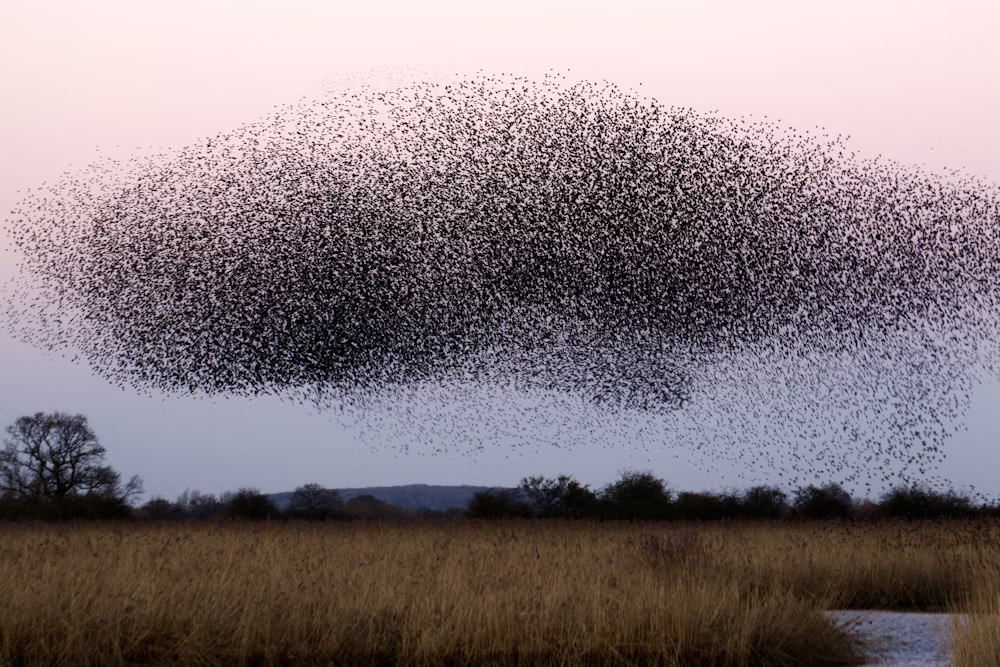
\includegraphics[width=\linewidth]{./bandadas_de_aves}
                        \label{fig:bandadas_de_aves}
                    \end{figure}
                \end{minipage}
            \end{frame}

        \subsection{Fundamentos}

            \begin{frame}{Fundamentos}
                \begin{itemize}
                    \item El modelo de Bandadas de Agentes Autopropulsados se basa en dos ecuaciones principales:
                        \begin{equation}
                            x_i(t+1) = x_i(t) + v_i(t) \Delta t\label{eq:equation1}
                        \end{equation}
                        \begin{equation}
                            \theta(t+1) = \langle \theta(t) \rangle_r+ \Delta \theta\label{eq:equation2}
                        \end{equation}
                    \item El $\langle \theta(t) \rangle_r$ es el promedio de los ángulos de las partículas vecinas:
                        \begin{equation}
                            \langle \theta(t) \rangle_r = atan2(\langle sin(\theta(t)) \rangle_r, \langle cos(\theta(t)) \rangle_r)
                        \end{equation}
                \end{itemize}
            \end{frame}

    \section{Implementación}

        \begin{frame}{Implementación}
            \begin{itemize}
                \item El modelo computacional se realizó en Java y cuenta con tres clases principales:
                \begin{itemize}
                    \item \texttt{MovingParticle}: representa una partícula en el espacio.
                    \item \texttt{OffLatticeAutomata}: representa el modelo de bandadas de agentes autopropulsados.
                    \item \texttt{Main}: clase principal que ejecuta la simulación.
                \end{itemize}
            \end{itemize}
        \end{frame}

        \subsection{Arquitectura}

            \begin{frame}{Diagrama UML}
                \begin{figure}[htbp]
                    \centering
                    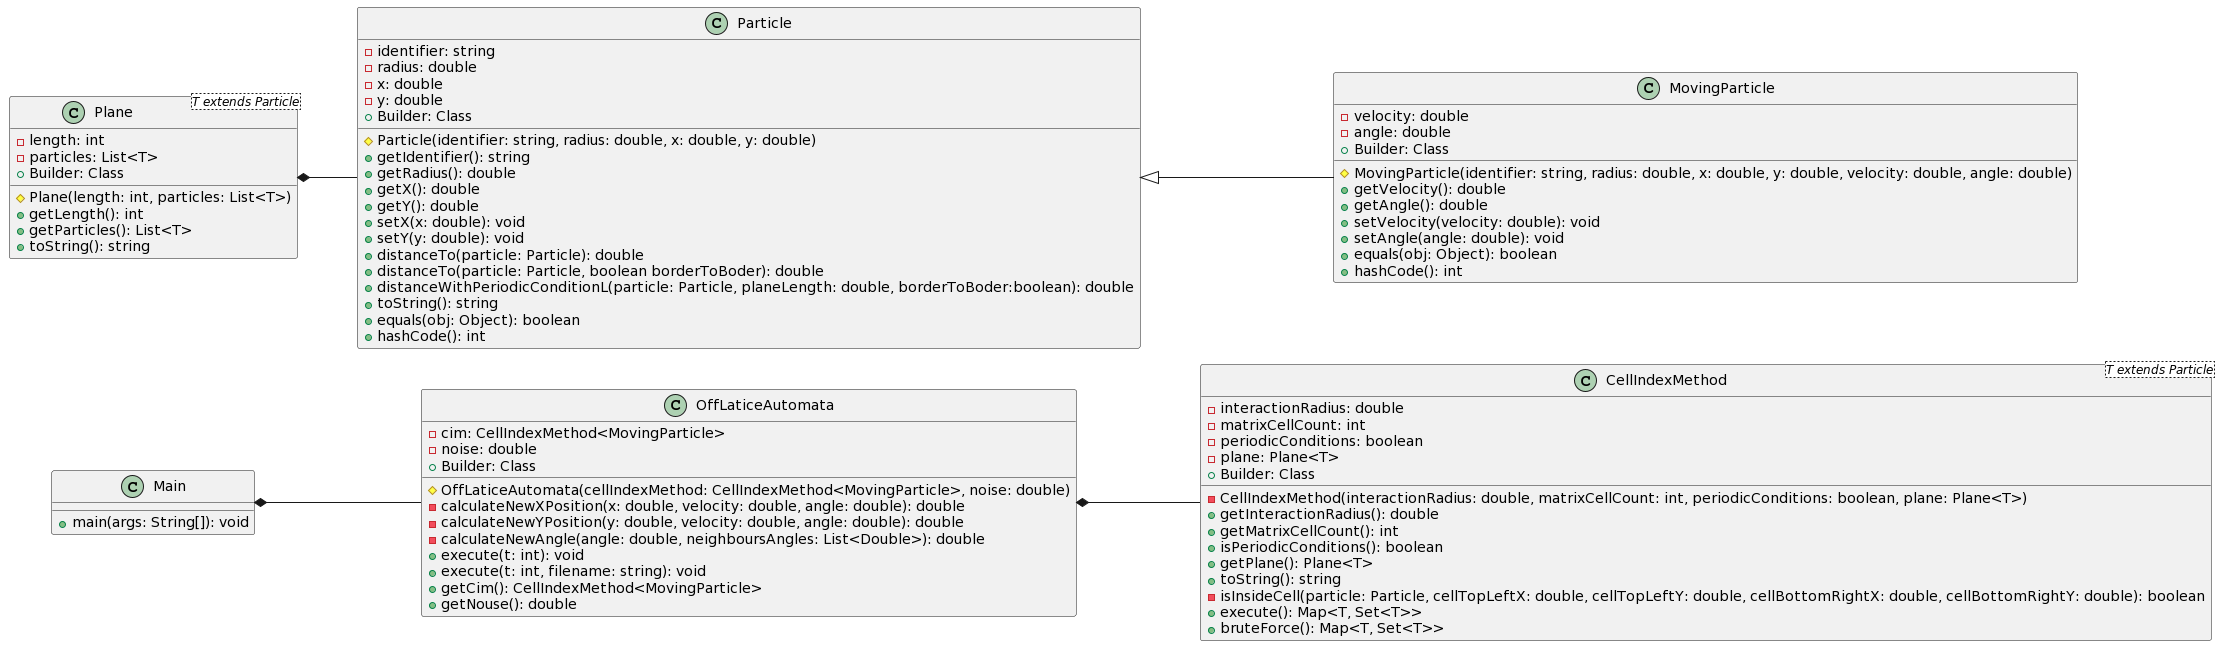
\includegraphics[width=\textwidth]{./architecture-landscape}
                    \label{fig:architecture}
                \end{figure}
            \end{frame}

        \subsection{Algoritmo}

            \begin{frame}{Pseudocódigo del algoritmo implementado}{}
%                {\fontfamily{consola}\selectfont
                    \begin{algorithmic}[1]
                        \ttfamily \footnotesize
                        \State Create output file
                        \While{$t < t_{max}$}
                            \State neighbours $\gets$ \Call{CellIndexMethod()}{}
                            \State list$_{\text{particle, angles}}$ $\gets$ \Call{Map}{neighbours}
                            \Comment{En $t$}
                            \ForAll{(particle, angles) $\in$ list}
                                \State $\theta_{\text{new}} \gets$ \Call{NewAngle}{particle, angles}
                                \State \Call{UpdateAngle}{particle, $\theta_{\text{new}}$}
                                \State \Call{UpdateXPosition}{particle, $\theta_{\text{new}}$}
                                \State \Call{UpdateYPosition}{particle, $\theta_{\text{new}}$}
                                \State Write output for $t$
                            \EndFor
                            \State $t \gets t + 1$
                        \EndWhile
                    \end{algorithmic}
%                }
            \end{frame}

    \section{Simulaciones}

        \subsection{Parámetros de entrada}

            \begin{frame}{Parámetros de entrada}
                \begin{itemize}
                    \item Parámetros de entrada fijos:
                    \begin{itemize}
                        \item $r_c$: radio de interacción. \alert{Se considera $r_c=1$}
                        \item $v$: módulo de la velocidad. \alert{Se considera $v=0.03$}
                        \item $L$: longitud del plano. \alert{Se considera $L=5$}
                    \end{itemize}
                    \item Parámetros de entrada variables:
                    \begin{itemize}
                        \item $N$: cantidad de partículas
                        \item $\eta$: ruido
                    \end{itemize}
                \end{itemize}
            \end{frame}

        \subsection{Salida de la simulación}

            \begin{frame}[fragile]{Archivo de salida}
                \begin{itemize}
                    \item Se genera un archivo \texttt{.txt} con la información de cada partícula, para cada tiempo
                \end{itemize}
                \begin{exampleblock}{Ejemplo}
                    \begin{verbatim}
0 p_0 4.204905 3.934431 -1.851475
0 p_1 2.606319 1.453672 -1.034532
0 p_2 4.460304 4.998664 -1.692054
...
597 p_179 3.054664 1.422251 1.905239
597 p_180 4.249935 2.057734 1.916287
597 p_181 4.204868 0.888108 1.815435
                    \end{verbatim}
                \end{exampleblock}
            \end{frame}

        \subsection{Observables}

            \begin{frame}{Parámetro de orden o polarización $v_a$}
                \begin{itemize}
                    \item Se define como:
                    \begin{equation}
                        v_a = \frac{1}{Nv} \left|\sum_{i=1}^{N} \vec{v_i} \right|
                    \end{equation}
                    \item Tiende a cero (0) cuando las partículas se encuentran en total desorden.
                    \item Tiende a uno (1) cuando las partículas se encuentran polarizadas.
                \end{itemize}
            \end{frame}

            \begin{frame}{Tiempo en el que el nro. de visitas alcanza el 20\% de $N$ }
                \begin{itemize}
                    \item Se define para las visitas en condiciones periódicas de contorno.
                    \item Se estudia su variación dependiendo de $\eta$ (ruido).
                    \item Como se tienen en cuenta cuatro $(4)$ zonas circulares fijas de visitas, es necesario promediar
                    los tiempos obtenidos de cada una de ellas y su error asociado:
                    \begin{equation}
                        t_{\text{prom}} = \frac{1}{4} \sum_{i=1}^{4} t_i \ ,\ t_i\text{: tiempo en la zona }i
                    \end{equation}
                \end{itemize}
            \end{frame}

            \begin{frame}{Número de visitas por unidad de tiempo}
                \begin{itemize}
                    \item Se define para las visitas en condiciones abiertas de contorno.
                    \item Se estudia su variación dependiendo de $\eta$ (ruido).
                    \item Se lo calcula como la pendiente de la curva de nro. de visitas en función del tiempo.
                    Se aplica el método de regresión lineal simple:
                    \begin{equation}
                        m_k = \frac{N \sum_{i=1}^N x_i y_i - \sum_{i=1}^N x_i \sum_{i=1}^N y_i }{N \sum_{i=1}^N x_i^2 - \left(\sum_{i=1}^N x_i \right)^2}
                        \ , 1 \leq k \leq 4
                    \end{equation}
                    \item Se promedian los valores obtenidos de cada una de las zonas y se calcula su error asociado:
                    \begin{equation}
                        m_{prom}(N,\eta) = \frac{1}{4} \sum_{i=1}^{4} m_i
                    \end{equation}
                \end{itemize}
            \end{frame}


    \section{Resultados}

        \subsection{Parámetro de orden $v_a$}

            \begin{frame}{Parámetro de orden $v_a$}{Animación}
                \begin{minipage}[t]{0.60\textwidth}
                    \begin{figure}[H!]
                        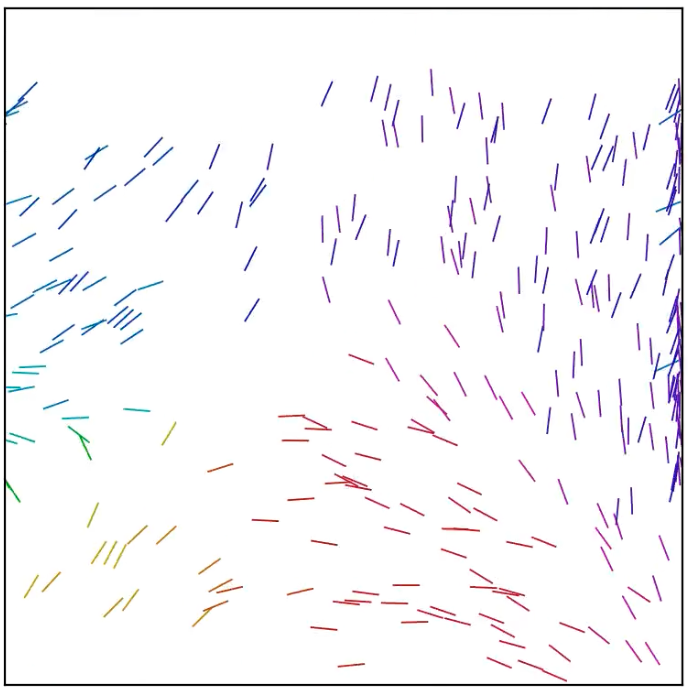
\includegraphics[height=.65\textheight]{./animation-n300-eta0p6-frame}
                        \caption*{Véase la animación completa en \url{https://youtu.be/q8ep24AgTzU}.}
                        \label{fig:va_1}
                    \end{figure}
                \end{minipage}
                \hfill
                \begin{minipage}[t]{0.30\textwidth}
                    \begin{block}{Datos del sistema}
                        \begin{itemize}
                            \item $N=300$
                            \item $L=5$
                            \item $\eta=0.6$
                        \end{itemize}
                    \end{block}
                \end{minipage}
            \end{frame}

            \begin{frame}{Parámetro de orden $v_a$}{Animación}
                \begin{minipage}[t]{0.60\textwidth}
                    \begin{figure}[H!]
                        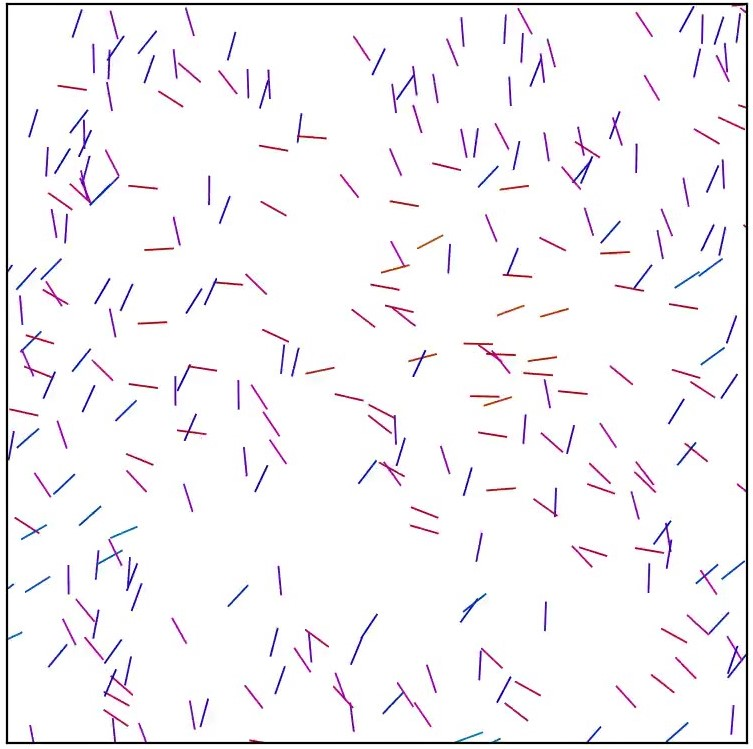
\includegraphics[height=.65\textheight]{./animation-n300-eta2p4-frame}
                        \caption*{Véase la animación completa en \url{https://youtu.be/aZ9eOtlXgQw}.}
                        \label{fig:va_2}
                    \end{figure}
                \end{minipage}
                \hfill
                \begin{minipage}[t]{0.30\textwidth}
                    \begin{block}{Datos del sistema}
                        \begin{itemize}
                            \item $N=300$
                            \item $L=5$
                            \item $\eta=02.4$
                        \end{itemize}
                    \end{block}
                \end{minipage}
            \end{frame}

            \begin{frame}{Parámetro de orden $v_a$}{Animación}
                \begin{minipage}[t]{0.60\textwidth}
                    \begin{figure}[H!]
                        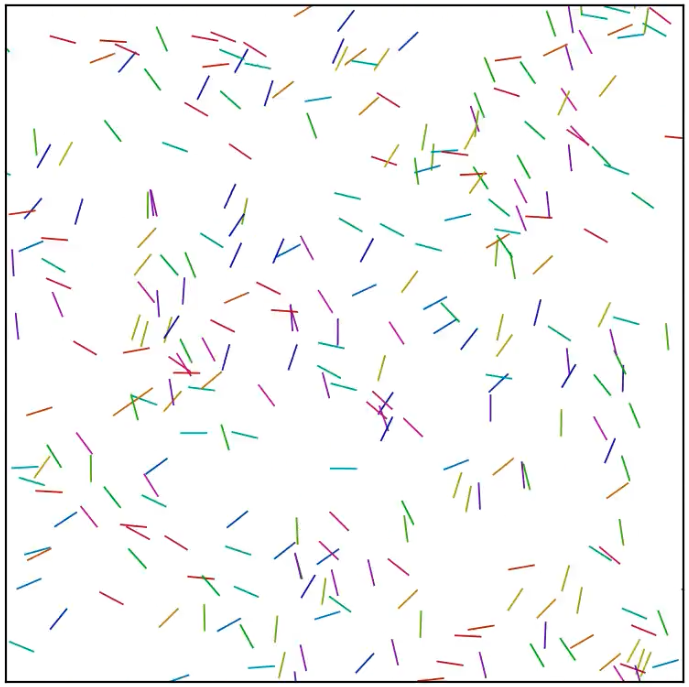
\includegraphics[height=.65\textheight]{./animation-n300-eta5p2-frame}
                        \caption*{Véase la animación completa en \url{https://youtu.be/QkXskl_8CGs}.}
                        \label{fig:va_3}
                    \end{figure}
                \end{minipage}
                \hfill
                \begin{minipage}[t]{0.30\textwidth}
                    \begin{block}{Datos del sistema}
                        \begin{itemize}
                            \item $N=300$
                            \item $L=5$
                            \item $\eta=5.2$
                        \end{itemize}
                    \end{block}
                \end{minipage}
            \end{frame}

            \begin{frame}{Parámetro de orden $v_a$}{$v_a$ en función del tiempo}
                    \begin{figure}[H!]
                        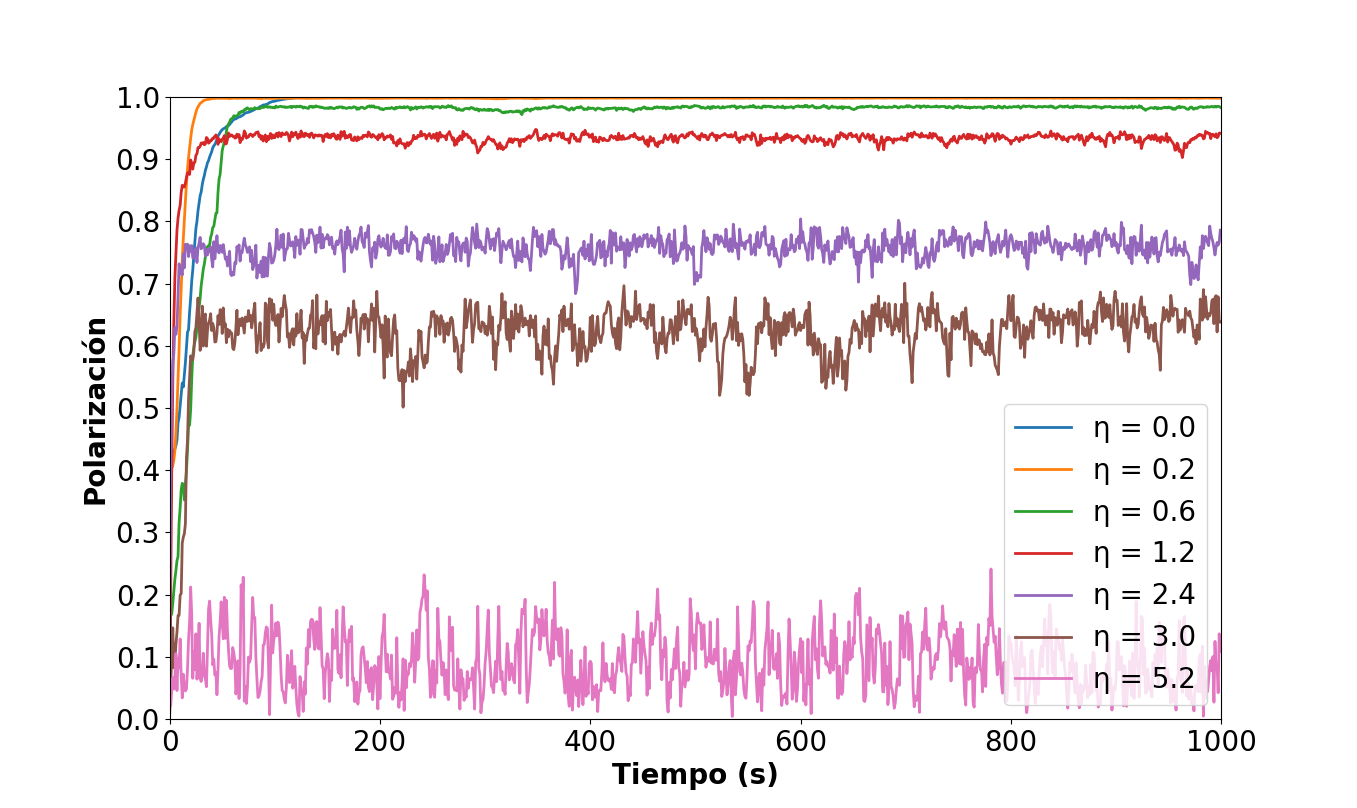
\includegraphics[width=0.9\textwidth]{./va_vs_time-n300}
                        \label{fig:va_4}
                    \end{figure}
                    \begin{beamercolorbox}[sep=5pt,center]{block body}
                        \begin{minipage}[t]{0.45\textwidth}
                            \centering
                            \small{$N=300$}
                        \end{minipage}
                        \hfill
                        \begin{minipage}[t]{0.45\textwidth}
                            \centering
                            \small{$L=5$}
                        \end{minipage}
                    \end{beamercolorbox}
            \end{frame}

            \begin{frame}{Parámetro de orden $v_a$}{$v_a$ en función del ruido ($\eta$)}
                \begin{figure}[H!]
                    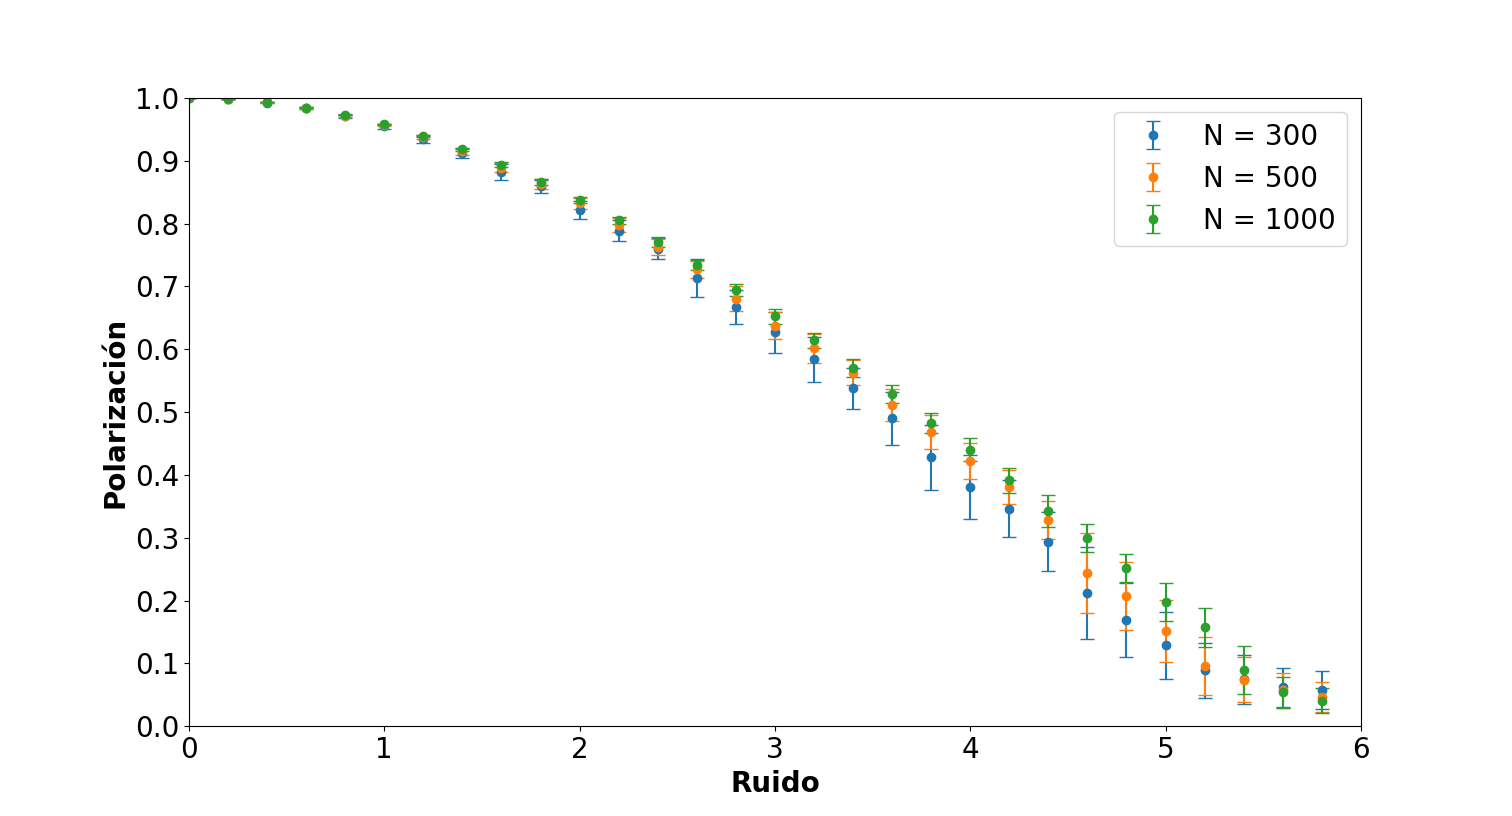
\includegraphics[width=0.9\textwidth]{./va_vs_eta}
                    \label{fig:va_5}
                \end{figure}
                \begin{beamercolorbox}[sep=5pt,center]{block body}
                    \small{$L=5$}
                \end{beamercolorbox}
            \end{frame}

        \subsection{Tiempo en el que el nro. de visitas alcanza el 20\% de $N$}

            \begin{frame}{Tiempo en el que el nro. de visitas alcanza el 20\% de $N$}{Animación}
                \begin{minipage}[t]{0.60\textwidth}
                    \begin{figure}[H!]
                        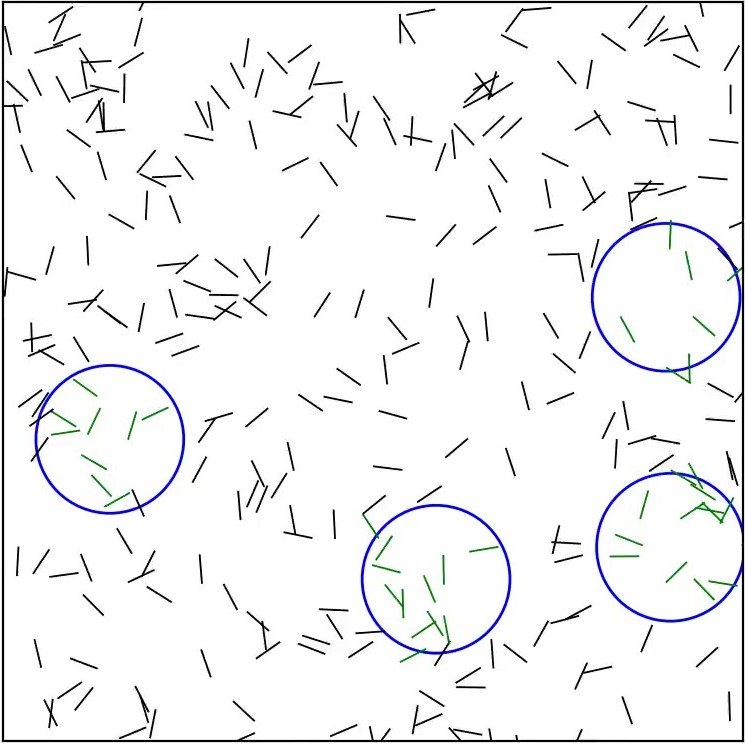
\includegraphics[height=.65\textheight]{animation_visits_pbc-n300-eta0p6-frame}
                        \caption*{Véase la animación completa en \url{https://youtu.be/MGHMlVLz0Ys}.}
                        \label{fig:pbc_1}
                    \end{figure}
                \end{minipage}
                \hfill
                \begin{minipage}[t]{0.30\textwidth}
                    \begin{block}{Datos del sistema}
                        \begin{itemize}
                            \item $N=300$
                            \item $L=5$
                            \item $\eta=0.6$
                        \end{itemize}
                    \end{block}
                \end{minipage}
            \end{frame}

            \begin{frame}{Tiempo en el que el nro. de visitas alcanza el 20\% de $N$}{Cantidad total de visitas en función del tiempo}
                \begin{figure}[H!]
                    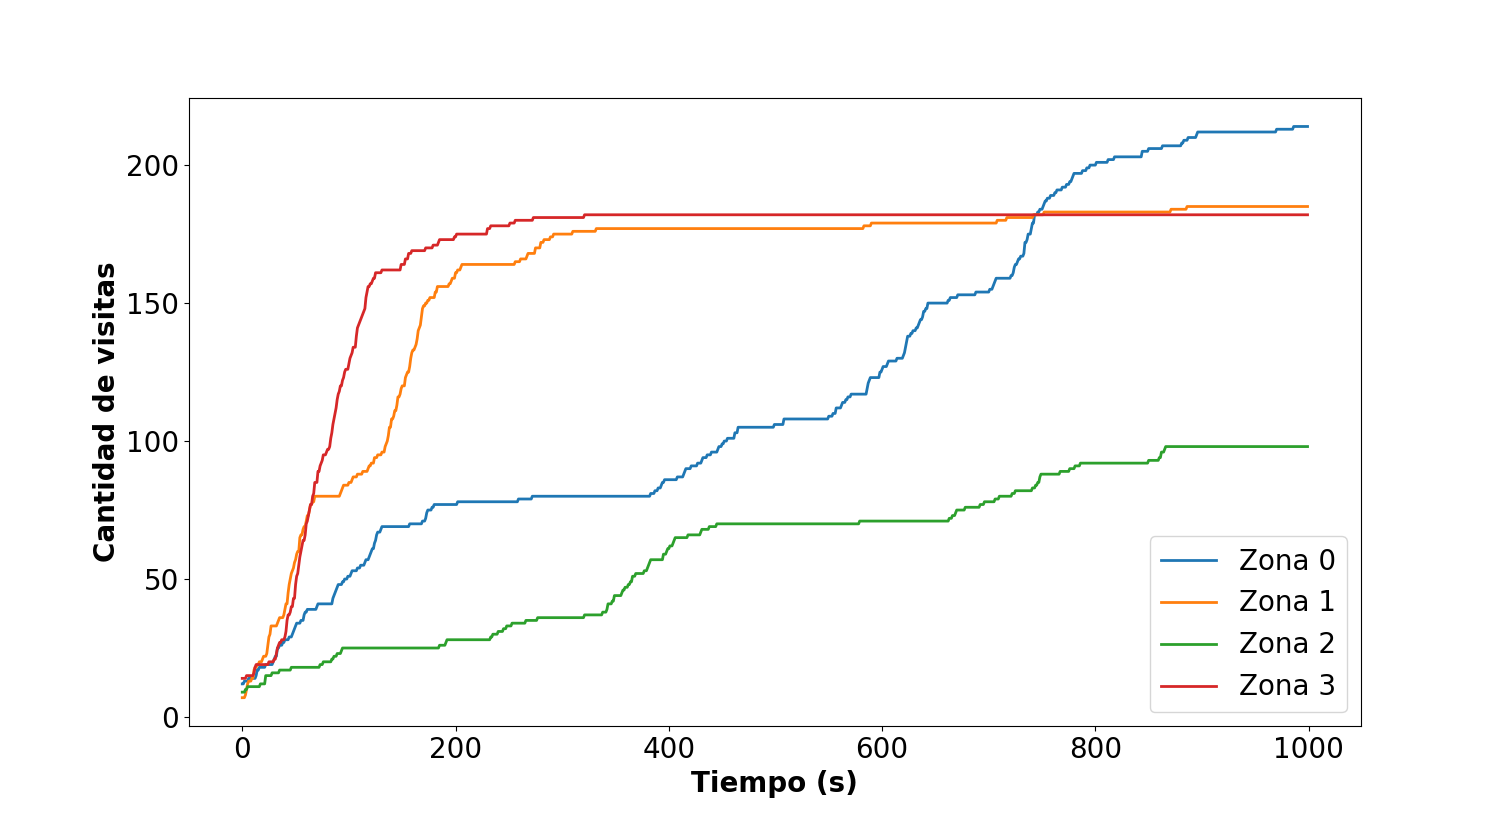
\includegraphics[width=0.9\textwidth]{./visits_vs_time_pbc-n300-eta0p6}
                    \label{fig:pbc_2}
                \end{figure}
                \begin{beamercolorbox}[sep=5pt,center]{block body}
                    \begin{minipage}[t]{0.3\textwidth}
                        \centering
                        \small{$N=300$}
                    \end{minipage}
                    \hfill
                    \begin{minipage}[t]{0.3\textwidth}
                        \centering
                        \small{$L=5$}
                    \end{minipage}
                    \hfill
                    \begin{minipage}[t]{0.3\textwidth}
                        \centering
                        \small{$\eta=0.6$}
                    \end{minipage}
                \end{beamercolorbox}
            \end{frame}

            \begin{frame}{Tiempo en el que el nro. de visitas alcanza el 20\% de $N$}{Observable en función del ruido ($\eta$)}
                \begin{figure}[H!]
                    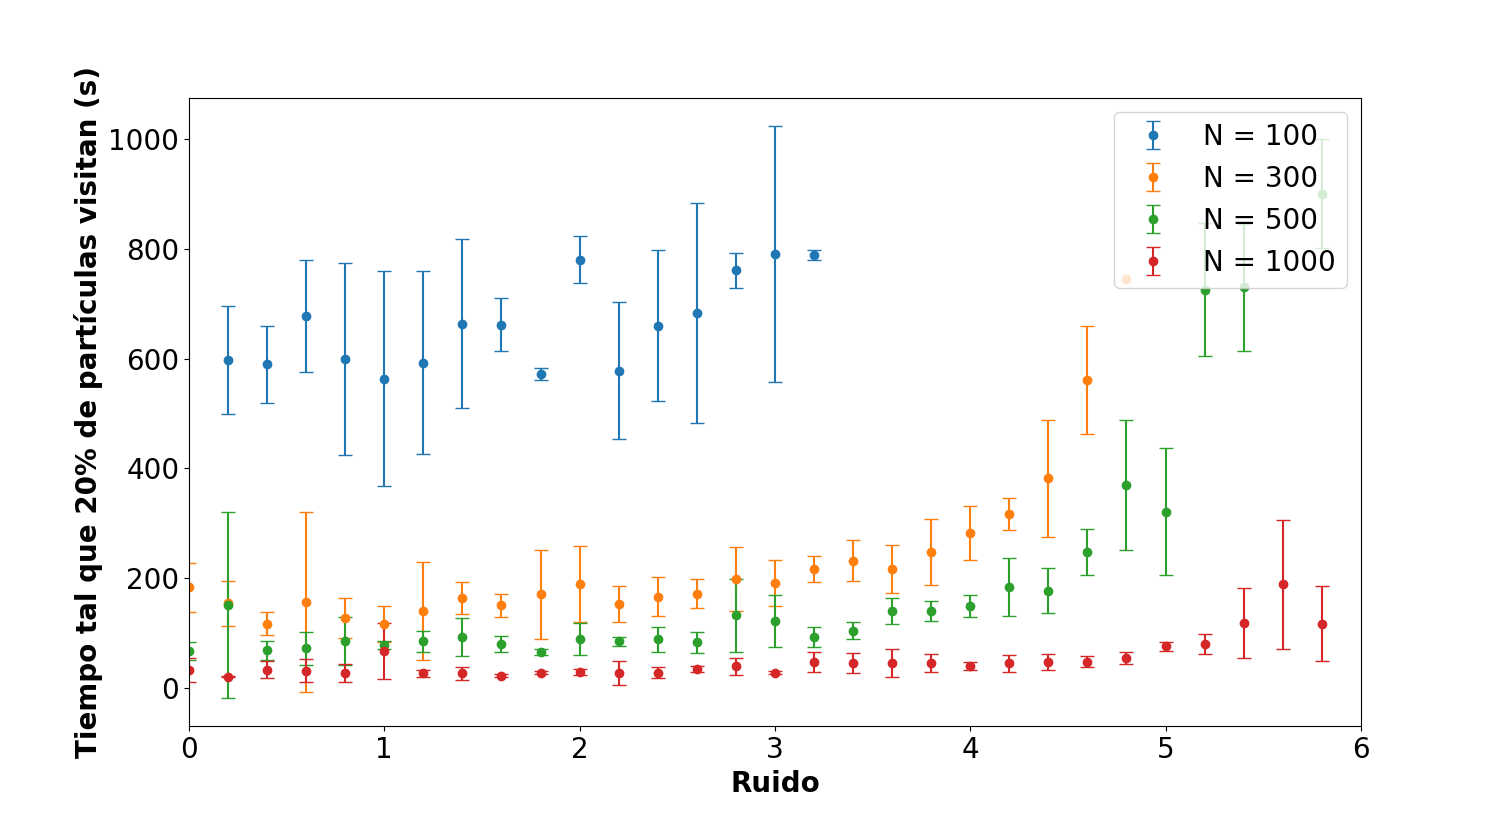
\includegraphics[width=0.9\textwidth]{./threshold_vs_eta-pbc}
                    \label{fig:pbc_3}
                \end{figure}
                \begin{beamercolorbox}[sep=5pt,center]{block body}
                    \small{$L=5$}
                \end{beamercolorbox}
            \end{frame}

        \subsection{Nro. de visitas por unidad de tiempo}

            \begin{frame}{Nro. de visitas por unidad de tiempo}{Animación}
                \begin{minipage}[t]{0.60\textwidth}
                    \begin{figure}[H!]
                        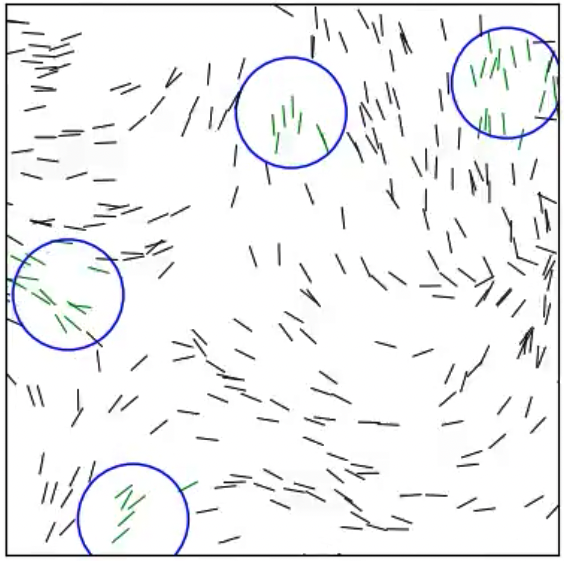
\includegraphics[height=.65\textheight]{./animation_visits_obc-n300-eta0p6-frame}
                        \caption*{Véase la animación completa en \url{https://youtu.be/ZcCPUwjMHBc}.}
                        \label{fig:obc_1}
                    \end{figure}
                \end{minipage}
                \hfill
                \begin{minipage}[t]{0.30\textwidth}
                    \begin{block}{Datos del sistema}
                        \begin{itemize}
                            \item $N=300$
                            \item $L=5$
                            \item $\eta=0.6$
                        \end{itemize}
                    \end{block}
                \end{minipage}
            \end{frame}

            \begin{frame}{Nro. de visitas por unidad de tiempo}{Cantidad total de visitas en función del tiempo}
                \begin{figure}[H!]
                    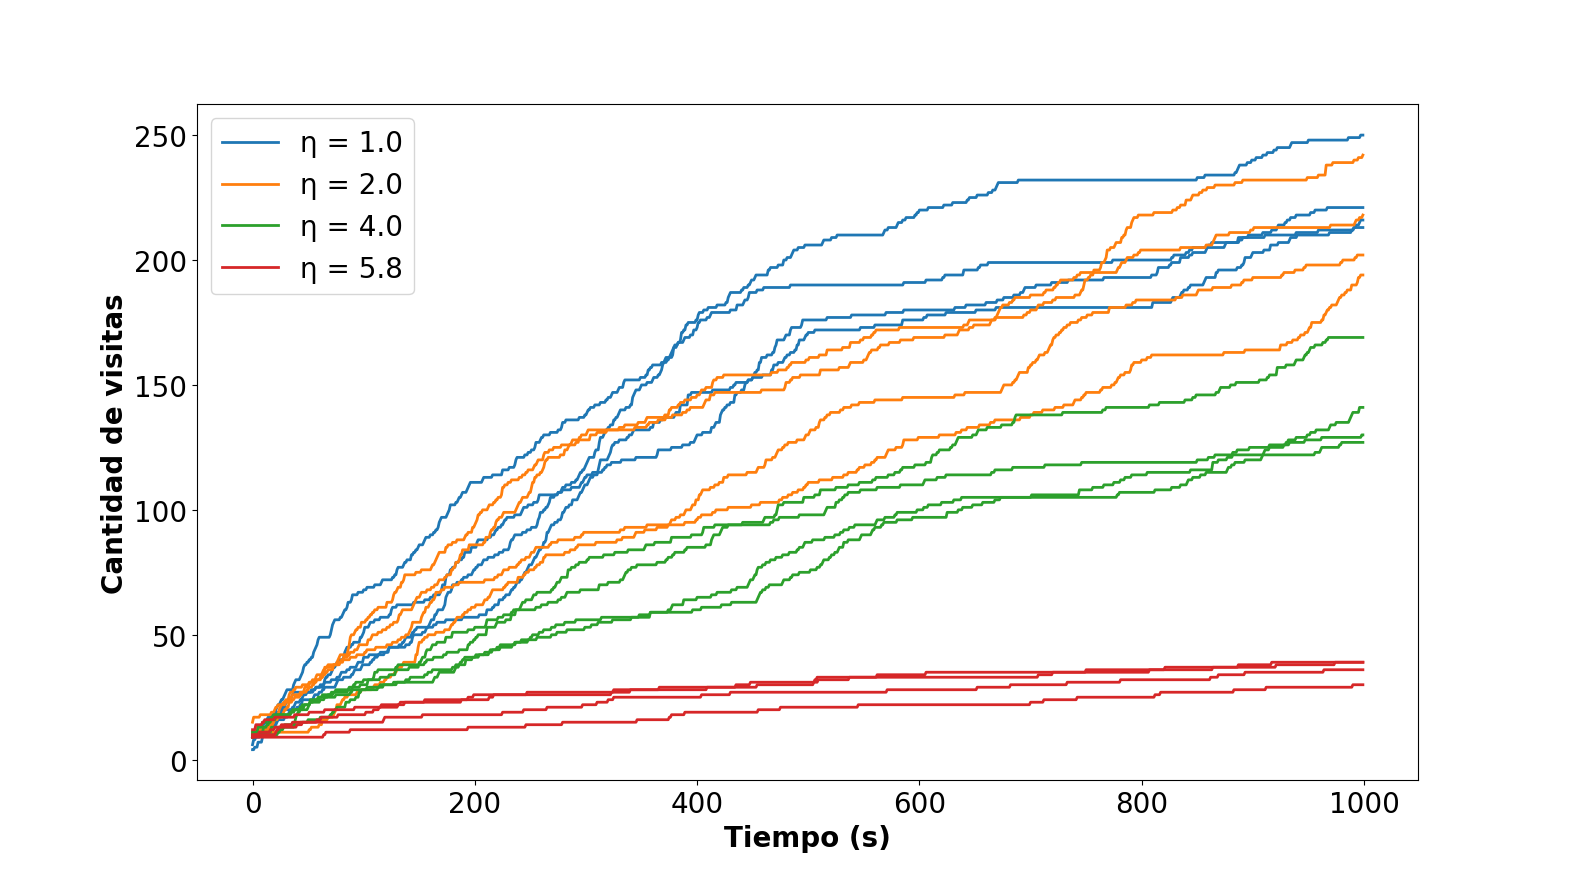
\includegraphics[width=0.9\textwidth]{./visits_vs_time_obc-n300}
                    \label{fig:obc_2}
                \end{figure}
                \begin{beamercolorbox}[sep=5pt,center]{block body}
                    \begin{minipage}[t]{0.45\textwidth}
                        \centering
                        \small{$N=300$}
                    \end{minipage}
                    \hfill
                    \begin{minipage}[t]{0.45\textwidth}
                        \centering
                        \small{$L=5$}
                    \end{minipage}
                \end{beamercolorbox}
            \end{frame}

            \begin{frame}{Nro. de visitas por unidad de tiempo}{Observable en función del ruido ($\eta$)}
                \begin{figure}[H!]
                    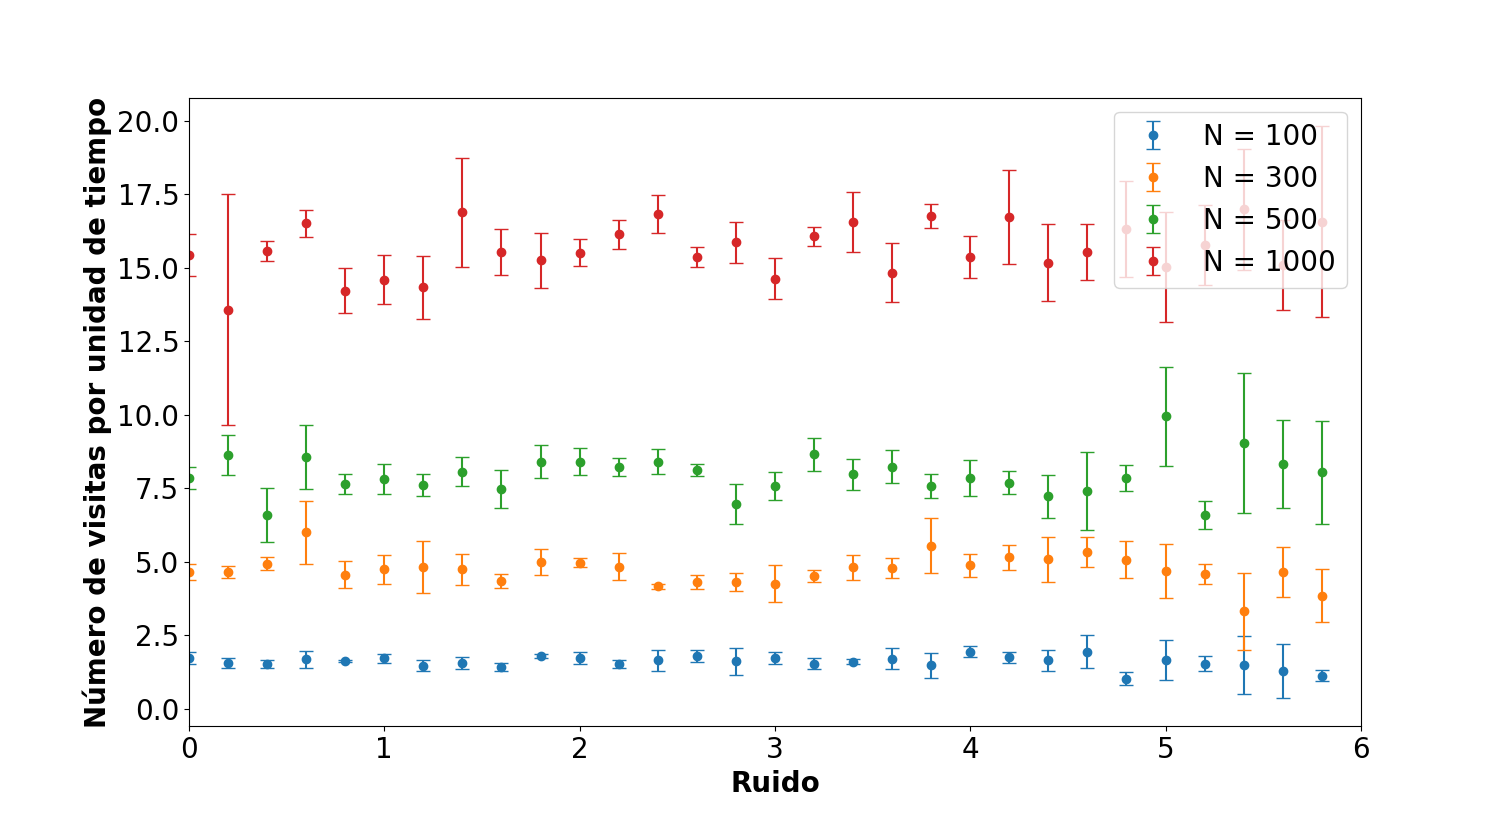
\includegraphics[width=0.9\textwidth]{./slope_vs_eta-obc}
                    \label{fig:obc_3}
                \end{figure}
                \begin{beamercolorbox}[sep=5pt,center]{block body}
                    \small{$L=5$}
                \end{beamercolorbox}
            \end{frame}

    \section{Conclusiones}

        \begin{frame}{Conclusiones}
            \begin{itemize}
                \item Se observó que a medida que aumenta la cantidad de partículas, la polarización tiende a ser
                levemente mayor
                \item En las visitas PBC se puede notar que:
                \begin{itemize}
                    \item a medida que el ruido se incrementa, el tiempo en el que el número de visitas alcanza un
                    porcentaje de $N$ también aumenta.
                    \item para valores de baja cantidad de partículas y/o alto ruido, no se alcanza ese umbral.
                \end{itemize}
                \item En las visitas OBC se puede contemplar que:
                \begin{itemize}
                    \item la cantidad de visitas por unidad de tiempo disminuye a medida que el ruido aumenta, sin importar el $N$.
                    \item para valores altos de $\eta$, la cantidad de partículas que visitan las zonas es acotada.
                \end{itemize}
            \end{itemize}
        \end{frame}

\end{document}
